\chapter{Constructing a Cardiac Simulation Toolkit}

\section{Simulation Environment}

The simulation environment provided by the cardiac toolkit is intended to be as
portable as possible, so that numerical experiments may be run on whichever
platforms are appropriate.  To this end, all the data input structures are based
on open standards, or simple binary formats.  The output formats provided by the
various driver programs are also in simple binary or ASCII formats, to allow
them to be easily visualized with both commercial and open source visualisation
tools.  The results presented later in this chapter were performed on desktop
computers with a XX GHz Althon X2 chip and 1 GB RAM and on Horace, the local HPC
facility.  Horace has 24 compute nodes, each one consisting of four Intel Itanium2
Montecito Dual Core 1.6GHz processors, 16GB RAM and up to 512GB of local scratch
space.  The nodes are connected by a high speed Quadrics QsNetII
interconnect~\cite{horace}.  Horace provides compilers for both Fortran and C,
and for both the MPI and OpenMP parallelization libraries.

\subsection{Implementation}

The experimental protocol drivers and the cellular models were implemented in
the C programming language, although much of the supporting code and
supplementary tools were implemented in the ruby programming language.  The
cellular models currently implemented are based on the Hodgkin-Huxley formalism,
although there is no fundamental reason why a Markov chain based model could not
be included.  Inter-cellular coupling for propagation of excitation over a
strand or tissue was implemented using the monodomain equations.

\subsubsection{Cellular Models}

The cellular model used for much of the developmental process was the
Courtemanche et al. human atrial myocyte model~\cite{crn98}.  Also currently
implemented are the Nygern et al. human atrial myocyte model~\cite{nygern98} and
the four variable formulation of the Fenton-Karma minimal variable
model~\cite{overo2008}.  These cellular models describe the behaviour of a cell
using coupled systems of non-linear ordinary differential equations.  The ODEs
represent the concentrations of intra- and extra-cellular ion species and the
flow of current through ionic channels in the cell membrane or between
intra-cellular compartments, or their notional equivalents in the case of minimal
variable models.

These equations were generally solved using the simplest time-stepping method
available, the explicit Euler method.  To improve performance and stability,
some variables were integrated using the Rush-Larsen method.  More complex
integration schemes were tried, but did not significantly improve performance to
compensate for the greater complexity.

\subsubsection{Monodomain Equations}

The monodomain equations were used to couple multiple cells together to describe
a tissue over which excitation could be conducted.


A discussion of the merits of the monodomain and bidomain equations can be found
in the introduction.


\subsubsection{Strand Model}

The 1D strand model is used for several experimental protocols, as
a computationally cheaper alternative to a full tissue model.  The 1D strand
model consists of a number of nodes, typically 200 or 300, which are coupled
electrically at the ends of the cells.  The electrical activity at each node is
modelled via a cellular electrophysiology model and electrical conduction between the
nodes is handled via a 1D formulation of the monodomain equations, with no
flux boundary conditions.

\subsubsection{Sheet Model}

The 2D sheet model is used for several experimental protocols, as well as more
general numerical experimentation.  The 2D sheet model consists of a grid of
nodes, coupled electrically along the cardinal directions of the grid.  The
electrical activity at each node is modelled via a cellular electrophysiology
model.  Conduction of the electrical excitation between the nodes uses the
mono-domain equations with no flux boundary conditions applied at all tissue
boundaries.  The square sheet model, used in several of the numerical
experimental protocols described later, is typically 375x375 nodes, representing
140625 cellular models.  Two dimensional idealizations of physiological
preparations can have many more nodes, to on the order of $10^{6}$ cellular
models.  These idealizations can often be quite irregular and so to allow easy
and effective partition of workload across multiple processors, the tissue map
is decomposed into a 1D array which contains references to the neighbouring
cells.


\subsection{Parallelization}

Some parts of the toolkit require the modelling of large numbers of cells, on
the order of tens or even hundreds of thousands of cellular models in two
dimensional sheets.  Solving all the equations involved takes a significant
amount of time and so it is desirable for such simulations to be parallelized so
that the work involved can be split over several processors.  This can have
advantages beyond merely having eight rather than one cores worth of
computational cycles working on solving the equations.  Splitting the work over
multiple cores can also increase the amount of cache available, allowing for
more efficient operation of the solvers.

For the toolkit, the OpenMP~\cite{OpenMP} parallelization library was chosen.
This implements the shared memory parallelism paradigm.  Using the shared memory
paradigm is simpler, due to the lack of explicit communication calls, and can be
faster, as there is merely memory access involved, rather than communication
over an network or other interconnect.  Finally, a program written using OpenMP
can, with some care, also be compiled serially if an OpenMP compiler is not
available.  Whilst a program implemented using a non-shared memory paradigm,
such as using the MPI library, would allow it to be executed on potentially more
processors which would potentially offer faster run times, in practice the eight
core shared memory system Horace provides as a compute node was general found to
be sufficient for the task.

\subsection{Optimisation}

The toolkit uses several techniques to optimize the computations performed,
reducing the number of processing cycles required to compute the results needed
for publication.  These optimisations are generally built around the principle
of ``No code is faster than no code'', although it might be more accurate to say
``No code execution is faster than no code executed''.  To explain this idea
another way, it is that no combination of compiler flags can compete with a
sensible choice of algorithm which minimizes the number of computational steps
to be performed or the amount of data to be written to a file.  This is not to
say that the compiler is are unimportant, but that it is merely the start of
optimisations, rather than the final step.

\subsubsection{The Compiler}

The toolkit has been compiled using the GNU C compiler (gcc)~\cite{gcc}, the
Intel C compiler (icc)~\cite{icc} and the Sun microsystems .  All three have
OpenMP implementations available and all three are capable of performing a
number of optimisations, controlled via flags.  The most important aspect of the
optimisations is that they should not alter the behaviour of the floating point
handling, as this could have significant impact on the final result computed.
Despite this caveat, the results of applying certain optimisation flags can be
quite significant.

\subsubsection{Caching of Computed Values}

Moving beyond the compiler, one of the simplest forms of optimisation is to only
calculate each value once, if at all possible.  This can be done in a number of
ways and the toolkit developed here implements two such methods for saving
computational time.

State saving is one of the most direct ways of caching computed values.  At a
particular point in the simulation, all of the state variables of the
system are copied into an intermediate location.  This might be a file on disk or
to another location in memory.  If the state is written out to a file, that file can
be used as a `save point', allowing the simulation to be continued from that
point in the future, ensuring work is not wasted.

When copied to another memory location, this allows the program to return to
that point in the future.  This is useful in modelling many experimental
protocols, which often call for a number of `conditioning' pulses to allow the
cell or model to settle.  The state can be saved after the conditioning pulses
and then the actual tests can be performed quickly, saving the execution of
several seconds of simulated activity.  This technique should obviously only be
used for cells in the Hodgkin-Huxley formalism which are deterministic and thus
give identical results whether the state is saved or not.  Using such a
technique with a cell that has a number of stochastic components could
potentially affect the quality of the results.

The second way in which caching can be employed is in the creation of `lookup
tables'.  A lookup table is a pre-computed table of the values an expression can
take.  When the expression would normally be evaluated, the table is used
instead, replacing what might be a complicated expression with a single array
lookup.  For lookup tables to be efficient to pre-compute, the tabulated
expression should depend on only one variable and should be sufficiently
`complex' expression, such as one involving the computation of mathematical logs
or exponentials.  The expression should depend on only one variable as the
pre-computed table has to be indexed over each variable the computation depends
on and even dependence on just two variables would increase the number of table
entries required by thousands or millions.  The requirement for complexity is a
little more obvious, as any optimisation can only save as much time as the
original series of operations took.  With these limitations in mind, it is still
possible to find many candidates for pre-computation in typical cardiac cell
models, most notably the activation and inactivations of voltage dependent
gates.  This technique is typically only worthwhile performing in the case of
tissue simulations where the benefits can be shared amongst all the cells since
pre-computation can be quite expensive, destroying any efficiency gains made
through their use for single cell simulations.

\subsubsection{Binary Searches}

Several of the experimental protocols provided by the toolkit are intended to
determine the value of a parameter which causes a particular condition to be
fulfilled, such as a successful excitation of the cellular model after
progressively shortening stimulus intervals.  This value we will call the
critical value. In real experiments, ones involving actual cardiac tissue, the
typical experimental protocol would involve stimulating the tissue at
sequentially shorter intervals, until no stimulation was provoked.  This might
involve stimulating the cell thousands of times, which would be expensive
computationally to model exactly.  Instead, a binary search for the critical
value can be performed, using the pseudo-code shown here.


To explain in words, first two guesses are made; the high guess, which is the
maximum value that the critical value can take, and the low guess, the minimum
it is presumed to take.  The simulation is then run with the parameter set at
the average of the low and high guesses--the current guess.  If the test is
successful, the critical value evidently lies somewhere between the low guess
and the average, and so the high guess is set to the current guess.  Conversely,
if the test is unsuccessful, the critical value is obviously above the current
guess, and so the low guess is set to the current guess.  The simulation is then
repeated with the average of the new high and low guess.  Using this algorithm,
the search space is halved with each iteration, swiftly finding the critical
value.  For example, to find a parameter somewhere in the range of 0--1000~ms to
the nearest millisecond requires just 10 iterations of the binary search
algorithm, but might take hundreds of iterations with sequential searching.

One important thing that must be considered when using binary searches is that
there is only one critical value in the range considered or else the algorithm
will give unpredictable results.  In practice, this limitation is often quite
easy to work within.

\subsubsection{Adaptive Step}

Adaptive step mechanisms are employed in the toolkit when there is a need to
provide output over a wide range of times, when the slope of the graph is not
constant over the range to be graphed.  This is very common in the modelling of
cardiac cells, which often show an exponential dependence of various parameters
on the  stimulus interval, and are graphed over a range of hundreds or thousands
of milliseconds.  A step that sufficient to track the curve at the upper limits
of the range will completely fail at the steeper slow of the lower limits,
whilst a step that will track the curve for the lower limits will result in
unnecessary work being done at the upper end of the range.  To alleviate this
problem, an adaptive stepping mechanism is used, as shown in this pseudo-code.

First, the measurement is performed at the largest desired point.  The interval
is then reduced by the step, and the measurement is performed again.  The
difference in the measurements is calculated and compared to the desired maximum
delta.  If the difference is acceptable, the interval is once more reduced by
the step, and the measurement taken once more.  If the difference is too great,
then instead the step size is halved and the measurement repeated.  If the
difference is now acceptable, then the interval is reduced by the new step and
the experiment proceeds.  If it is not, then the step size is once more halved.
The step size used is therefore always appropriate to the slope of the curve and
a smooth graph results.  Additional logic, not shown in the pseudo-code, is used
to ensure the step size does not become too small, and to terminate the graph at
the lower end of the range.

Since curves can increase or decrease the absolute difference between the two
values is compared.

\subsubsection{Parallel Input/Output}

Input and output for simulations is obviously essential if they are to be of any
use.  This input and output can involve the reading or writing of many megabytes
or gigabytes of information over the course of a simulation, often in a variety
of different formats.  This most significant for sheet simulations and it is
those that we consider here.

Data input is typically not that significant a cost for
simulations, as whilst various simulation maps and saved states be quite large,
the cost is typically only paid once.  Data output is often required at numerous
points throughout the course of the simulation since almost all simulations are
performed to examine the time evolution of the cardiac system.  Many simulations
will output the value of state parameters, most commonly the voltage, at all
points in the tissue every few milliseconds of simulated time.  Other state
variables might also be desired and the toolkit also offers `live visualization'
of two dimensional sheets via output of images in the GIF format.  In addition,
the whole state is output regularly, to allow simulations to be resumed at a
later point in time.  This output usually stops all simulation whilst it is
being written to disk, time during which the processors are typically idle.  By
allowing multiple threads to output in parallel, the cost of outputting multiple
files can be reduced to the cost of outputting one.


\section{Experimental Protocols}

The toolkit developed provides a number of experimental protocols to use with
the cellular models to quantify the electrophysiological behaviour of the
modelled cells.  The provided protocols include the action potential duration at
90\% repolarisation (APD90) and the action potential (AP) profile; the
APD90 and APD50 restitution; the effective refractory period (ERP) restituion
(ERPr); the conduction velocity (CV) restitution (CVr); the temporal
vulnerability window to unidirectional conduction block (VW) and a flexible
system for specifying two dimensional sheet experiments, including the
initiation of re-entry via wavebreak protocols and computation of the spatial
vulnerability window.

\subsection{Action Potential Duration}

\subsection{Action Potential Duration Restitution}

The toolkit calculates the APDr via a standard S1--S2 protocol used in both
numerical simulations and also in physiological experiments.  The APDr is used
as a measure of how the cell responds to stimulations at different rates.  The
protocol used is shown here.


The cellular model is paced nine times with a stimulus close to the threshold
value at a given frequency or BCL.  At this point, the state is saved for the
paced cells.  The tenth S1 stimulus is then given, followed by the S2 after a
varying DI, which is reduced via an adaptive step to record the relationship
between DI and the APD of the following AP.  The toolkit also determines useful
parameters such as the maximal slope of the restitution curve, which can be
related to the stability of spiral waves within the tissue.  Both the APD90 and
the APD50 restitution can be calculated.

\subsection{Effective Refractory Period Restitution}

The ERPr is calculated by the toolkit using standard experimental protocols.
The ERP is defined as the shortest possible stimulus interval which still allows
for a successful AP.  A successful AP is defined as an AP which has an amplitude
of at least 80\% of the magnitude of a normal AP.  To determine the rate
dependence of the ERP, it is evaluated at a decreasing BCL.


The cellular model is paced seven times, and then the state is saved just before
the eighth AP is initiated.  The ERP for each chosen pacing rate is found via
binary search.  The low guess is typically chosen as zero, whilst the high guess
is the BCL being tested.  The eight AP is initiated immediately and then the S2
stimulus is delivered at the average of the guesses, as described previously.
If the ninth AP is successful, in addition to updating the high guess, the S2
interval is stored in a `best guess'.  With this small alteration, the binary
search algorithm is performed as described, with the saved state restored after
each iteration.

The reduction in BCL is stepped via an adaptive mechanism.  The BCL is reduced
until it is sufficiently short that the stimuli are occurring within the tail end
of the AP.

\subsection{Vulnerable Window}

The VW is principally a tool of numeric experimentation, based around a 1D ring
model of cardiac arrhythmia.  The VW is defined as the time period after a
stimulation during which a second stimulus elicits unidirectional propagation
along the strand.  In the case of a ring this causes retrograde propagation
which cycles endlessly.  If the stimulus is given too early, then the tissue
will still be refractory and no propagation of excitation will ensue.  If it is
given too late, then propagation will occur in both directions, which in the
ring case, results in the two excitation wavefronts annihilating each other.
Normal pacing could then resume.

The VW is found in a 1D strand model, set up as described previously.  The
strand is 200 units long and with a space step of \mm{0.1}.  The first stimulus is
given to a 3 unit (\mm{0.3}) section at one end of the strand.  The test stimulus
is given to a 4 unit (\mm{0.4}) section, usually centred in the middle of the
strand. The VW is bounded on the lower side at the time when a stimulus any
earlier would result in no propagation from a test stimulus, and on the upper
side at the time when a stimulus any later would result in bidirectional
propagation from a test stimulus.  These three cases (no, unidirectional,
bidirectional) propagation are illustrated in figure TODO.

By counting the number of APs which cross the two ends of the strand--2, 3 and
4, respectively, for the three cases in figure TODO--the result of the test
stimulus can be determined.  The two boundaries of the VW are found via binary
search, with a lower guess of \ms{0} and an upper guess of \ms{1000}.  First, the
upper bound of the VW is determined by searching for the delay when 3 APs
crossing the ends becomes 4.  The lower bound is then found by looking for the
delay at which 3 APs crossing the ends of the strand become 2.  A minor
optimisation is performed when looking for the upper bound, in that the lower
bound's high and low guesses are updated at the same time, reducing the total
space which must be searched in the second half of the program.  Before the test
stimulus is administered, the strand may be pre-paced a number of times.  In
this case the strand state is saved as the middle of the strand is depolarized
and then restored for each binary division.

\subsection{Threshold of Excitation}

The threshold of excitation is a theoretical measure, proposed by Zhang et
al.~\cite{Zhang2003}\ and used in modelling studies~\cite{Kharche2008}.  It is
defined as the minimum stimulus current which, when delivered to a cell, will
cause the cell to depolarize to a membrane potential of at least \mv{-20}.  The
threshold of excitation is calculated for a range of stimulus intervals,
successively reducing the interval until it is impossible to elicit a
depolarization of sufficient magnitude.  At each stimulus interval it is
recorded if the test pulse elicits bidirectional, unidirectional or no
propagation.

The threshold of excitation is found in a 1D strand model.  The strand is 300
units long, with a space step of \mm{0.1}.  The strand is first given $N$ S1
stimuli at a rate which allows the strand to recover between each excitation
wave.  Each S1 stimulus is delivered to the first 4 nodes (\mm{0.4}) and is
chosen to be above the threshold of excitation.  The threshold of excitation is
calculated at the 100th node and so as this node depolarises, the state for the
whole strand is cached.

The threshold of excitation is then found via binary search, with a lower bound
of \unit{0}{nS} and an upper bound chosen to be 5x the normal threshold.  The
test stimulus is delivered $\Delta t$\ seconds after the 100th node depolarises
to a group of 4 nodes centred on the 100th node.  After the test stimulus is
delivered the 4 nodes are tested for the excitation condition, attaining a
membrane potential of \mv{-20}.  If it is successful, the current stimulus
strength will assigned to the high guess.  If not, to the low guess.  In
addition, the simulation is continued to evaluate whether bidirectional,
unidirectional or no conduction of the excitation wave is evoked by the
stimulus.  The strand is then reset to the cached state and the new stimulus
strength is tested until a sufficient accuracy has been attained.  Once the
threshold of excitation has been determined for a given $\Delta t$\ the state of
the strand is once more reset to the cached state and a shorter $\Delta t$\
tested.

\subsection{Conduction Velocity Restitution}

Measurement of CV (or solitary wave velocity) itself is performed both
experimentally and numerically, as is the minimum conduction interval, which is
the shortest interval between an S1 and an S2 stimulus which still travels the
length of the strand.  This is similar to the ERP, but can also be influenced by
factors which affect the inter-cellular coupling as well as heterogeneity in the
strand.  The CV\emph{r} provides both the solitary wave velocity, the CV for a large S2
interval and the minimum stimulus interval, when the S2 interval gets too short
for an excitation wavefront to be fully propagated.

The CV\emph{r} is found in a 1D strand model, set up as described previously.
The strand is 300 units long with a space step of \mm{0.1}.  Stimuli are
delivered to a 4 unit (\mm{0.4}) length at one end of the strand at a strength
above threshold.  The strand is first given $N$\ S1 stimuli at rate which allows
the strand to recover between their application.  The S2 stimulus is then
delivered $\Delta t$\ seconds later. The conduction velocity is estimated from
the time taken to propagate between two points 100 nodes from each of the ends
of the strand, to minimize the influence of boundary effects.  The S2 time is
then stepped via an adaptive step, until a second excitation wave does not
propagate the length of the strand.


\subsection{Spiral Wave Life Span}

Spiral Wave LS is examined experimentally and numerically.  The LS of the spiral
wave and the meander pattern of the tip are both used to gain insight into the
behaviour of the tissue under conditions of cardiac arrhythmia.

Spiral waves are initiated in a square sheet of tissue $375\,\text{x}\,375$
nodes in dimension with a space step of \mm{0.1}, as described previously.  The
tissue is first stimulated along one edge via a stimulus current applied to a
row of nodes extending the length of the tissue and 3 nodes (\mm{0.3}) in width.
The planar wave is then allowed to propagate over the tissue.  Some time after
the first wave is initiated, a second stimulus is applied.  The second stimulus
is applied to half the tissue, bisecting the first wave's propagation front.
The second stimulus is a voltage clamp, with all the included tissue clamped to
a `high' potential, typically \mv{+20}--\mv{+50} for a millisecond.  The
generated spiral is then allowed to evolve until it self-terminates, the spiral
wave tip exits the tissue or until a sufficient amount of time has passed such
that the spiral can be classified as `persistent'.  The time allowed for a wave
to be classified as persistent is typically 5 or \unit{10}{s}.

The spiral wave tip traces are calculated via a standard contour based
algorithm, comparing the \mv{-60} contour line on snapshots of the electrical
activity \ms{2.5} apart.

\subsection{Spatial Vulnerability Window}

The SVW is examined both experimentally and numerically.  It is used together
with the (Temporal) VW for quantifying a mutation or condition's potential for
arrhymogenesis.  It is defined as the smallest area of tissue in a 2D sheet,
which when given a threshold stimulus in the wake of a conditioning pulse causes
at least one `figure of eight' re-entry.  A figure of eight re-entry occurs when
the excitation waves from the tips of the test area propagate back through the
centre of the area, resulting in a pair of contra-rotating spiral waves at each
end of the region.

The sheet model used for the determination of the SVW can vary in size, as the
SVW can vary substantially, depending on the electrophysiology being simulated
by the cellular models at the nodes, but the smallest used is typically
$375\,\text{x}\,375$ nodes, with a spatial resolution of \mm{0.1}.  The sheet is first given one
conditioning excitation, initiated by injecting a strip of nodes 3 nodes
(\mm{0.3}) in width with current along one edge of the sheet.  The wave is then
allowed to propagate through the tissue.  When the VW of the tissue is
positioned at the centre of the tissue, the test stimulus is delivered.  The
test stimulus is an area of tissue 20 nodes (\mm{2}) wide and of variable length.
After the test stimulus is delivered, the sheet is observed until figure of
eight re-entry is observed, or it is obvious that it will not occur.  The
protocol is then repeated with a test stimulus area of greater length.


\section{Results From Simulation Studies}

The cardiac simulation toolkit has been used in several simulation studies.
Here I present two such studies, representing different aspects of the toolkit.
The first is based on an experimental study which determined the existence of a
novel ion channel in the human atrium which caries an anion current through the
cellular membrane.  The second is principally a 2D study, concerning the effects
of Atrial Fibrillation induced Electrical Remodelling (AFER) and
electrophysiological heterogeneity in a 2D idealization of the right atrium and
the sino-atrial node.

\subsection{Anion Currents In The Human Atrium}

\subsubsection{Introduction}

In a recent experimental study, Li et al.~\cite{li2007} determined the existence
of a novel outwardly rectifying anion current in human atrial myocytes isolated
from right atrial appendages taken from patients undergoing coronary bypass
surgery.  They determined that it was separate other known ionic currents and
performed preliminary modelling based on the CRN Human Atrial Myocyte
model~\cite{crn98}.  They determined the current could be modelled by
equation~\ref{anion:eqn} with the constants given in table~\ref{anion:table}.

The total current carried by the channel, \ii{ANION}, was given by

\begin{equation}
\label{anion:eqn}
I_{ANION} = g_{ANION} \frac{V-E_{ANION}}{1-\left(c\times e^{\left(V-E_{ANION}\right)}\right)}
\end{equation}

where $g_{ANION}$ is the conductivity of the anion channel, $E_{ANION}$ is
the reversal potential of the channel and $c$ and $d$ are constants to
describe the behaviour.  All other symbols have their usual meanings.

\begin{table}
    \caption[Parameter sets for the anion sensitive current]{
        Parameter sets for the anion sensitive current \ii{ANION}\ when carrying
        \nothree\ and $\text{Cl}^{\text{-}}$\ ions.
    }
    \begin{tabular}{ l  c c}
    \label{anion:table}
    & \nothree & $\text{Cl}^{\text{-}}$ \\
    \hline
    $g_{ANION}$ & 0.37   & 0.19 \\
    $E_{ANION}$ & -45.64 & -45.64 \\
    $c$         & 0.87   & 0.94 \\
    $d$         & $8.4\,\text{x}\,10^{\text{-4}}$ &  $2.5\,\text{x}\,10^{\text{-4}}$
    \end{tabular}
\end{table}


The simulation study used the parameter set for the anion current carrying
\nothree ions.  The effects of the addition of this current to atrial
myocyte cells was quantified .  In the following
paragraphs, `control' is used to denote the unmodified CRN model and `anion' to
denote the CRN model with the additional current described by (\ref{anion:eqn})
with the \nothree\ parameter set from Table \ref{anion:table}.

\subsubsection{Results}

The AP generated by the control and anion simulations are shown in
figure~\ref{anion:ap}.  The \apd\ is relatively unchanged, but is slightly
reduced from \ms{299.6} to \ms{298.0}, whereas the \apd[50]\ is significantly
reduced, from \ms{180.1} to \ms{160.1}.  The AP profile shows a depressed plateau region (phase
2), reduced from \mv{-9.56}\ to \mv{-14.1}\ and a slightly elevated resting potential,
\mv{-79.0}\ in the anion case cf. \mv{-80.9}\ in control.  This duplicates the Li et
al.~\cite{li2007} study, and is included here only for completeness.

\begin{figure}
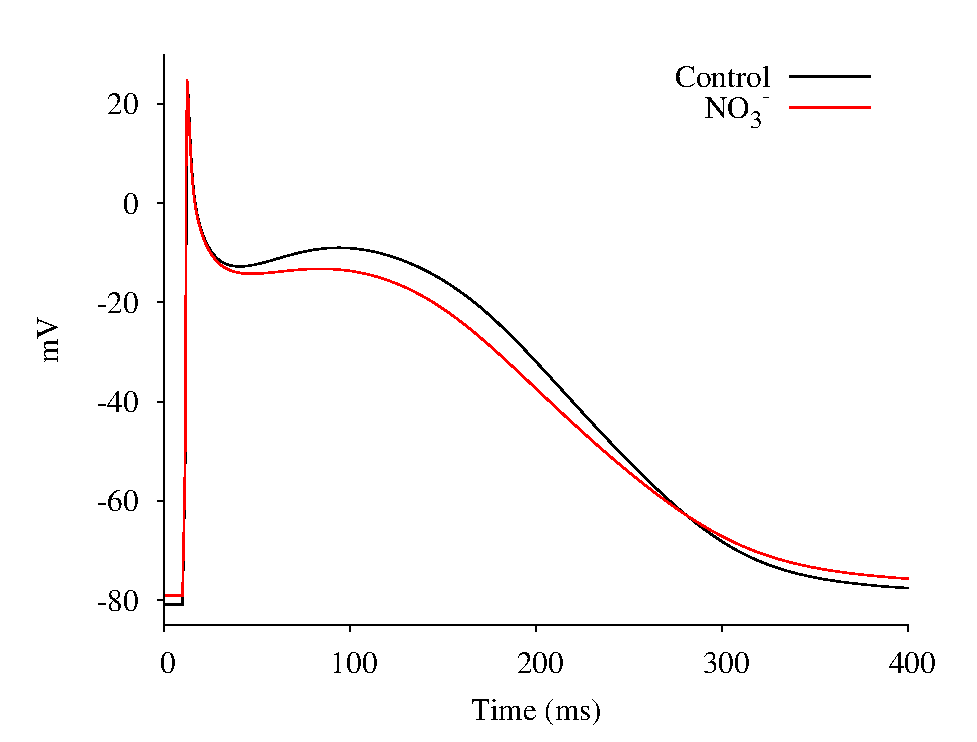
\includegraphics{figures/toolkit/anion/01_AP}
\caption[Anion Sensitive AP Profile]{\label{anion:ap} AP profile for the CRN
model in control (black) and anion (red) cases.  The inclusion of the
$NO_{3^{-}}$ carrying current results in a small change of AP morphology, with
a depressed plateau potential and an elevated resting potential.}
\end{figure}

The APDr curves produced by the control and anion cases are shown in
figure~\ref{anion:apdr50} and \ref{anion:apdr90}, for the restitution of APD at
50\% (\apdr[50]) and 90\% (\apdr) of repolarization, respectively.  The
\apdr[50]\ shows the most significant differences, with the anion
curve depressed by \ms{20} even at the largest DI, increasing to a maximum
difference of over \ms{40} at at DI of \ms{380}.  The two curves then rejoin each
other before they cross over at a DI of \ms{200}.  The \apdr\ curves, by
contrast, are very similar for control and anion cases at large (> \ms{600}) DI.
Between \msrange{100}{400}\ DI, the anion case is depressed compared to the control
case, with a difference of up to \ms{25}\ observed in the measured APDs.  At
\ms{100}, the curves rejoin one another and show a rapidly increasing slope as the
DI approaches \ms{0}.  In this region, the observed maximal slopes are XXX in
control and XXX in anion case.

\begin{figure}
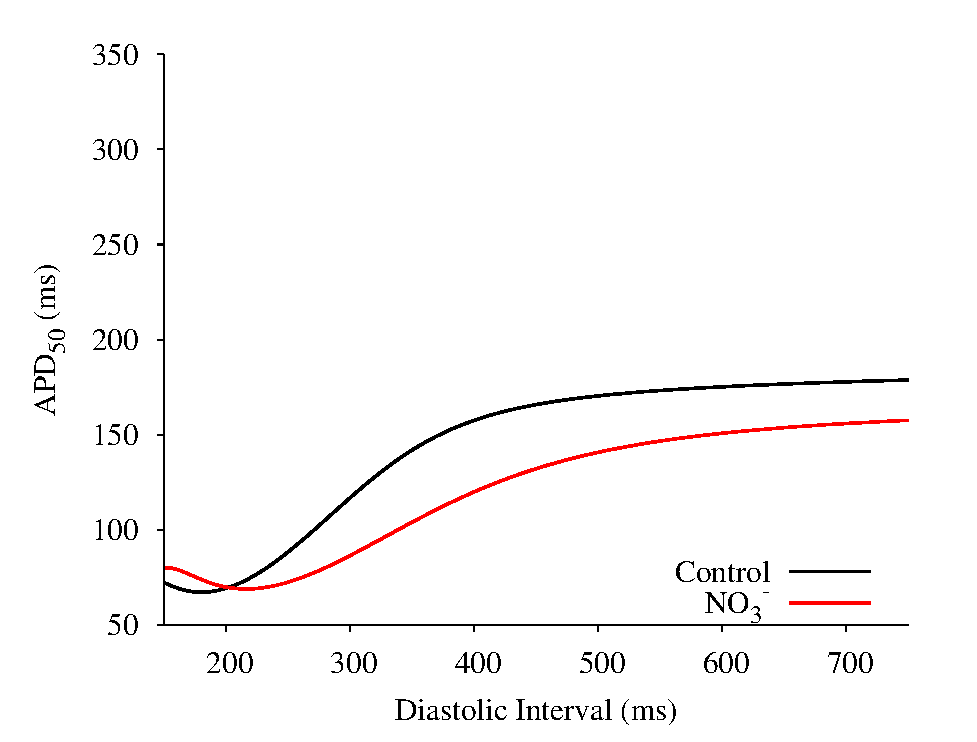
\includegraphics{figures/toolkit/anion/03_S1S2_50}
\caption[Anion Sensitive APD Restitution at 50 repolarization]{
\label{anion:apdr50} APDr curves for the CRN model in control (black) and anion
(red) cases at 50\% repolarisation.  The two variants are clearly different for
all the DI tried in the simulation, with the anion case considerably below the
control case for much of the DI tried.  The anion case also shows a reduced
slope of the restitution curve compared to the control case.  Note the
cross-over of the curves at a DI of \ms{200}.}
\end{figure}

\begin{figure}
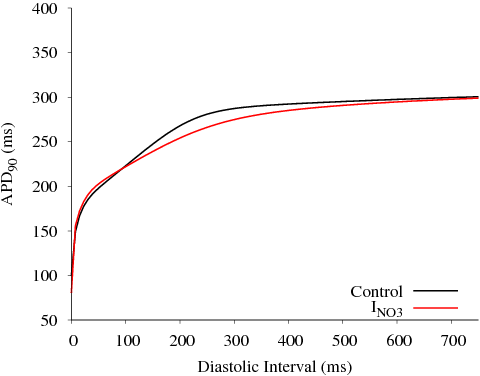
\includegraphics{figures/toolkit/anion/02_S1S2_90}
\caption[Anion Sensitive APD Restitution at 90 repolarization]{
\label{anion:apdr90} APDr curves for the CRN model in control (black) and anion
(red) cases at 90\% repolarisation.  The two variants behave the same at large
DI, but as the DI before the S2 stimulus is decreased, the anion case shows a
greater reduction in the \apd.  At short DI (below \ms{100}) the two curves
rejoin each other.}
\end{figure}

The ERPr curves produced by the control and anion cases are shown in
figure~\ref{anion:erpr}.  In both cases the ERPr curves are relatively flat,
decreasing by approximately \ms{50}\ over the \ms{500}\ range of BCLs considered.  The
addition of the anion current increased the ERP at all the BCLs considered in
the simulation by \msrange{10}{15}.  At very short BCLs (below \ms{400}), the shortest BCL
that can still produce an effective excitation is \ms{25}\ shorter for the control
compared to the anion cases.

\begin{figure}
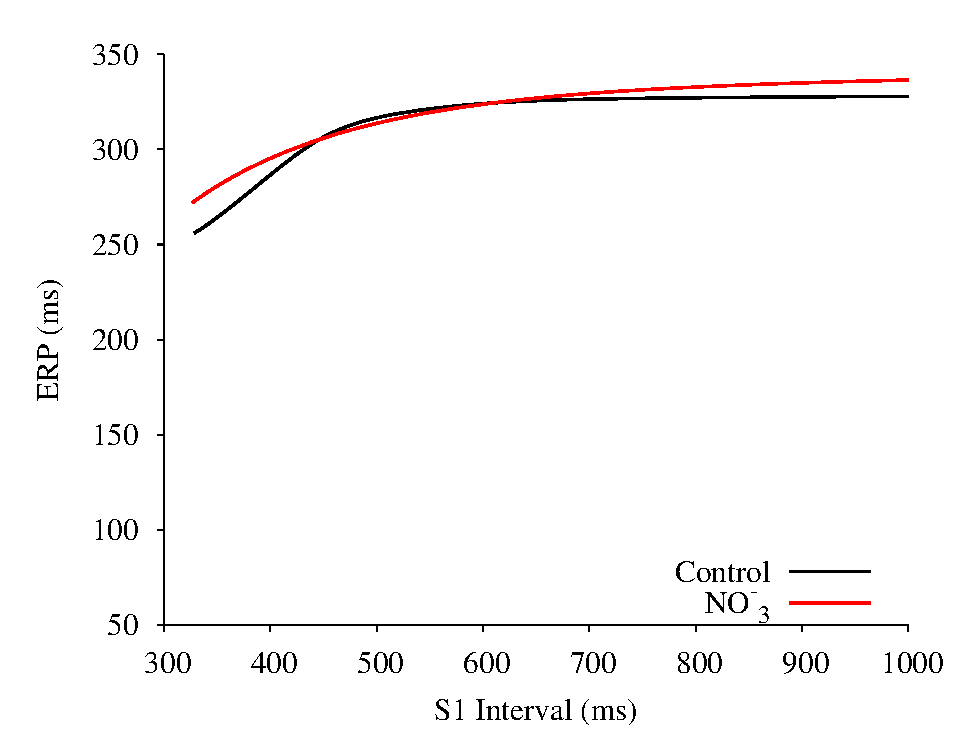
\includegraphics{figures/toolkit/anion/04_ERPR}
\caption[Anion Sensitive Effective Refractory Period Restitution]{
\label{anion:erpr} ERPr curves for the CRN model in control (black) and anion
(red) cases.  The ERPr curves are relatively flat for both cases.  The ERP is
always greater for the anion case.  In addition, the control case allows
successful excitation after pacing at 25~ms shorter BCL.}
\end{figure}

The temporal VW increased with the addition of the anion current from
\ms{6.7} in
control to \ms{7.3}\ in anion case, a 10\% increase in the size of the region of
unidirectional conduction block.  The CVR curves, shown in
figure~\ref{anion:cvr}, suggest that tissue with the anion sensitive current
shows faster CV at normal physiological stimulus intervals (corresponding to
\msrange{500}{1000}), with an average conduction velocity of
\cms{27.1}\ in anion, compared with \cms{26.7}\ in control.  As the conduction
interval is reduced below \ms{500}, the conduction velocity starts to decrease
rapidly until conduction stops at \ms{340} for anion and \ms{320} for control.

\begin{figure}
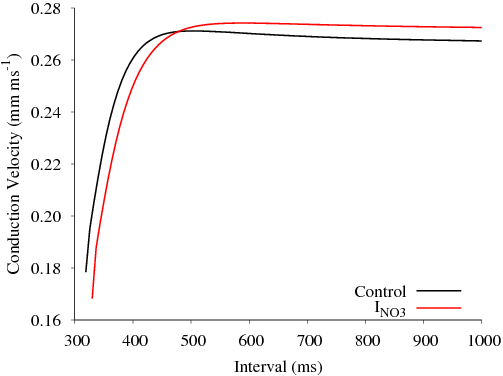
\includegraphics{figures/toolkit/anion/06_CV}
\caption[Anion Sensitive Conduction Velocity Restitution]{
\label{anion:cvr} CVr curves for the CRN model in control (black) and anion
(red) cases. The CVr curves are relatively flat for both cases over the range of
\msrange{500}{1000}, before they both increase rapidly in steepness until the minimum
stimulus interval is reached at approximately \ms{325} for both control and anion.
The CV is higher at longer stimulus intervals for the anion case, before it
crosses the control curve at a stimulus interval of \ms{475}.}
\end{figure}

Spiral waves were induced in a square $375\,\text{x}\,375$\ node sheet at a
resolution of \mm{0.1}, for a sheet dimension of \mm{37.5}\ per
side.  Representative plots of the membrane potential over the whole sheet,
produced as the simulation was ongoing, are show in figure~\ref{anion:spiral}.
Panels A i--iv show the membrane potential for control, whilst Panels B i--iv
show the membrane potential for anion, as the simulation evolved.  The path
followed by the spiral wave tip as it meandered is shown in A,v and B,v for
control and anion, respectively.  In both cases the spiral wave starts in the
centre of the tissue and then follows a looping track around the tissue before
finally it exits the tissue when it cannot turn fast enough around its own
refractory tail.  This process takes \ms{1700} in control and \ms{2300} in
anion.

\subsubsection{Discussions and Conclusions}

The effects of the inclusion of an anion sensitive current do not seem to be
that large, at least when considered on the single cell level.  This is perhaps
to be expected, as a current which did have a significant influence on the
action potential would surely have been identified sooner.  However, despite the
current's small influence on the action potential duration, it does have
significant effects on the restitution properties of the cell and on the
behaviour of cells in a tissue.

The most noticeable effect of the inclusion of \ii{ANION}\ in a cellular model
is the abbreviation of the \apd[50]\ and the accompanying reduction in the
plateau potential.  The abbreviation is due to \ii{ANION}\ acting as a
rectifying current when the membrane potential is above \mv{-45}.   Conversely,
at potentials below \mv{-45}\ \ii{ANION}\ acts to depolarize the cell, leading
to the slightly elevated resting membrane potential observed between action
potentials.  This difference in effect is what leads to the interesting
behaviours observed in cells with \ii{ANION}.

The \apdr[50]\ and \apdr\ curves show that \ii{ANION} has a rate dependent
effect.  Both curves are flattened in the cells which include \ii{ANION}\, but
this flattening is not uniform over the range of S2 intervals considered.
\ii{ANION}\ has a simple exponential dependence on the membrane potential and no
gating variables however, so it is not \ii{ANION}\ which causes this rate
dependence directly.  Instead, we must look to the currents active within the
plateau region of the action potential.  \ii{CaL}\ is the principle current
responsible for the plateau region of the action potential and unlike \ii{ANION}
it has both an activation gate, $d$, and an inactivation gate, $f$.  The $d$\
gate is not as interesting as the $f$\ gate, as its time-course is not affected
by the presence of \ii{ANION}, although its activation during the plateau region
is reduced.  Conversely, the $f$\ gate in \ii{ANION} cells never inactivates as
completely as it does in the control simulations which lack the current.




\subsection{Atrial Fibrillation Induced Remodelling And Heterogeneity}

\subsubsection{Introduction}

The human atria consists of several tissue types each with distinct
electrophysiological properties.  It has previously been shown that
inhomogeneity in tissues can lead to re-entrant activity
\cite{Bernus2005, Coronel1992, Kumagai1997}.  There is also experimental
data available on the ion channel remodelling due to atrial
fibrillation induced remodelling (AFER) during chronic atrial
fibrillation (AF) on human atrial cells~\cite{Bosch1999,Workman2001}.

In this study, we quantified the changes in electrophysiological
behavior in cell and 1D homogeneous models under AFER compared to control
conditions.  Further, re-entrant waves in 2D electrically homogeneous
and electrically heterogeneous sheets were studied.

\subsubsection{Methods}

The human atrial action potential (AP) model by Courtemanche et
al.\cite{crn98} was used in this study.  Modifications were
incorporated to reproduce the differing APs of the different atrial cell
types~\cite{Seemann2006}.  This produced distinct APs for the
crista terminalis (CT), pectinate muscles (PM), atrio-ventricular ring
bundle and the Bachmann bundle.  Atrial myocyte (AM) cells were modelled
by the original CRN model.

The data for AFER were taken from experiments by Bosch et
al.~\cite{Bosch1999} and Workman et al.~\cite{Workman2001}, representing
the changes in ion channels in patients after one month (AF1)
and up to six months (AF2) of chronic AF, respectively.  The
modifications to the cellular electrophysiology were described in
Kharche et al.~\cite{Kharche2007}.

The effects of AFER were quantified through a variety of measures.  The
\apdr\ and the \apdr[50]\ were calculated
as described in .  There were 9 S1 stimuli at a frequency of
\unit{1}{Hz}, followed by a varying DI after~\cite{blah2009}.  The ERP\emph{r}
was calculated as described previously, with 7 S1 delivered at the given pacing
rate and then a final S2 stimulus was used to determine the ERP after Workman et
al.~\cite{Workman2001}.  The VW and the CV\emph{r} were determined for control,
AF1 and AF2 conditions, for each of the three atrial cell types classified by
Seemann et al.. There were therefore nine 1D strand models tested.  The strand
models were each 200 nodes long, with a spatial resolution of \mm{0.1}.  The
diffusion constant used for all simulations was set to
$0.03125\,\text{mm}^{\text{2}}\,\text{ms}^{\text{-1}}$~\cite{Biktasheva2005},
giving a solitary wave conduction velocity of
$0.267\,\text{mm}\,\text{ms}^{\text{-1}}$\ in control atrial tissue.  In all 1D
strand simulations there was 1 S1 pulse and one S2 pulse.  This pulse was
applied over 4 nodes (\unit{0.4}{mm}), had duration \ms{2} and magnitude
\unit{10}{nS}.

Further, a 2D electrically heterogeneous sheet model was developed based on a
laboratory photograph of the right atrium.  The photograph was digitized at a
spatial resolution of \mm{0.1}. The model developed by segmenting areas of the
tissue into AM, PM and CT tissue types.  The complete model had a size of
$130\,\text{x}\,100\,\text{mm}$ and consisted of approximately 1 million active cell nodes.  The
simulations were performed with all cells under control, AF1 and AF2 conditions,
with the conditions applied uniformly to the tissue.  All 2D sheet simulations
were performed with the space step of \mm{0.1} and a time step of \ms{0.05}.

\subsubsection{Results}

Simulations were performed for all three cases: control, AF1 and AF2.
However the results for AF1 and AF2 were qualitatively similar, although
AF1 showed a much more profound effect on \apd\ reduction.

Incorporating the heterogeneity and AFER data causes significant
differences in \apd\ to manifest, as shown in Figure~\ref{fig:apdr}. The
effects of AFER are not uniform across the different cell types of the
atrium and it increases the difference in \apd\ between normal atrial
myocytes and the CT cells, increasing from \ms{20.1} in control to \ms{28.1}
in AF1 and \ms{33.4} in AF2.

The APD\emph{r} curves, shown in Figure~\ref{fig:apdr}, are flatter over much
of the range of diastolic intervals for AF1 and AF2 as compared to
control.  However, the maximal slopes
of the APDr curves for CT cells are higher for AF1, 5.3, and AF2, 2.8,
compared with 2.1 in control.  The difference in the maximal slopes in
different tissue types is increased, with CT having a larger maximal
slope in all cases.  In the control tissue, the difference in maximal
slopes was 0.1, compared with 0.4 in AF1 and 0.5 in AF2 tissue.

\begin{figure}[tb]
\centering
%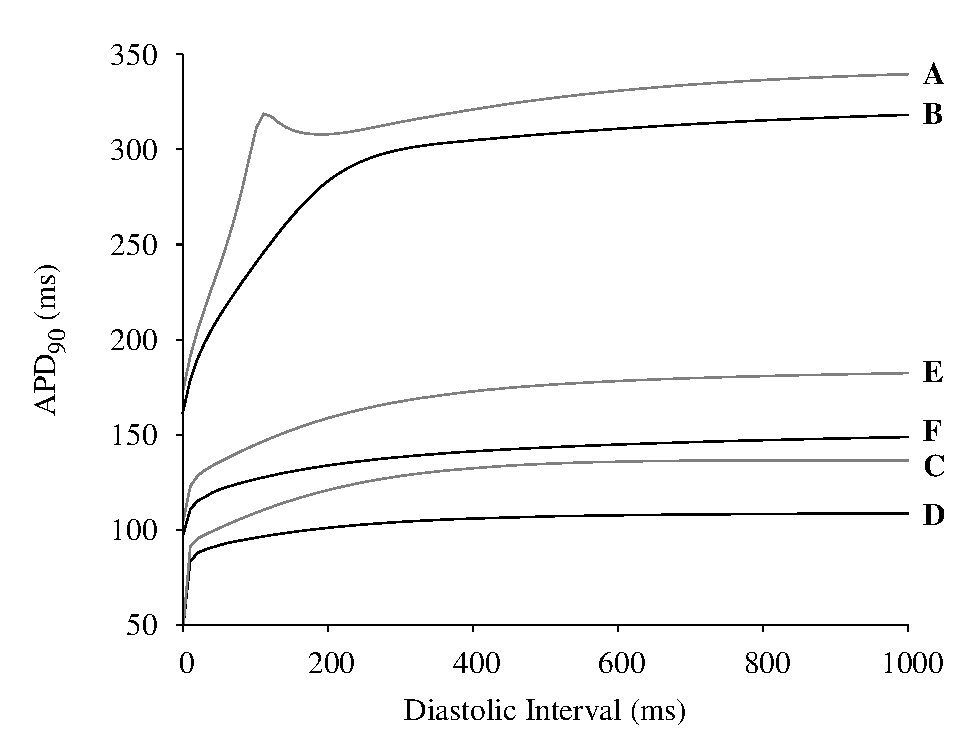
\includegraphics{figures/2_apdr}
\caption{APDr curves for control CT (A), control AM/PM (B), AF1 CT (C),
AF1 AM/PM (D), AF2 CT (E), AF2 AM/PM (F). In all cases the CT action
potentials are above the AM/PM action potentials over the whole of the
range considered.}
\label{fig:apdr}
\end{figure}

In AF tissue, the ERP\emph{r} was flattened for all tissue types compared with
the control cells, as shown in Figure~\ref{fig:erpr}.  The curves also extended
to lower BCLs for AF tissue, indicating that it was possible to excite AF tissue
successfully at a higher rate than was possible in control tissue.
Heterogeneity in ERP\emph{r} was largely unaffected by AF.

\begin{figure}[tb]
\centering
%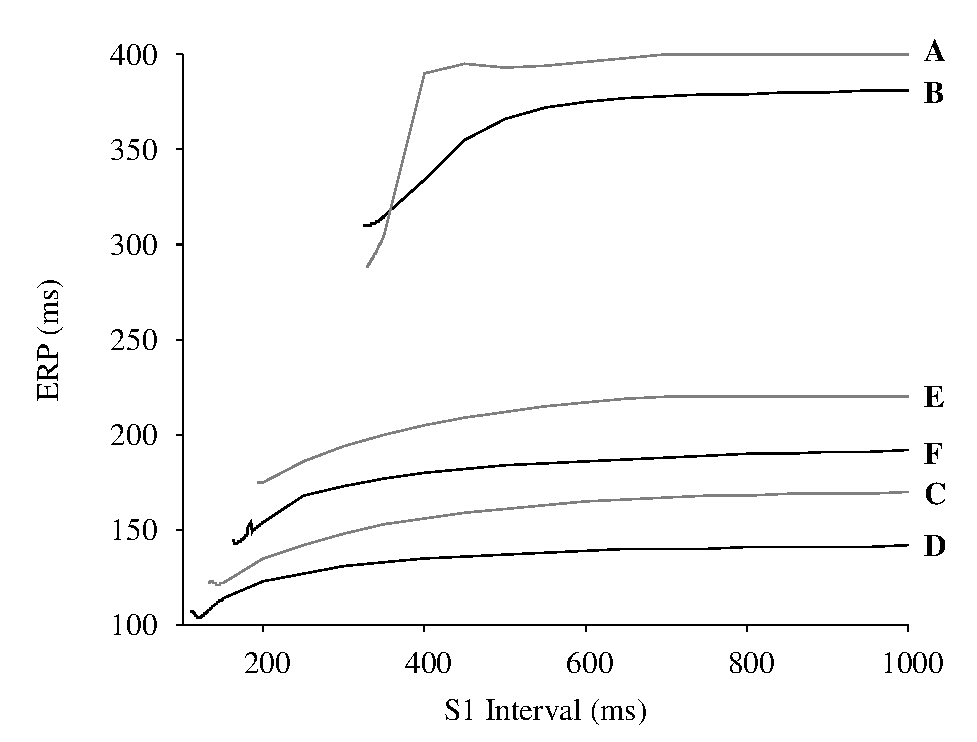
\includegraphics{figures/3_erpr}
\caption{ERPr curves for control CT (A), control AM/PM (B), AF1 CT (C),
AF1 AM/PM (D), AF2 CT (E), AF2 AM/PM (F).  Both AF1 and AF2 have a
significantly reduced ERPr over the whole range considered, with AF1
having a lower ERP then AF2.  In addition, AF1 and AF2 cells are still
excitable after pacing at \ms{100} shorter BCL.}
\label{fig:erpr}
\end{figure}

Conduction velocity, shown in Figure~\ref{fig:cvr}, was slowed by AF,
reducing the solitary wave velocity from $0.27\,\text{mm}\,\text{ms}^{\text{-1}}$\ in
control to $0.25\,\text{mm}\,\text{ms}^{\text{-1}}$\ in AF1 and
$0.26\,\text{mm}\,\text{ms}^{\text{-1}}$\ in
AF2.  Maximal pacing rate increased from the control value of \unit{198}{bpm} to
\unit{421}{bpm} in AF1 strands and \unit{315}{bpm} in AF2 strands.

The VW was reduced by AF, but in all cell types the reduction was small.
The control value of \ms{16.6} was reduced to \ms{14.2} in AF1 and \ms{14.7}
in AF2 for AM and PM cell types.  The reduction in VW for CT cells was
even smaller, from \ms{15.1} in control to \ms{14.5} and \ms{14.4} in AF1 and
AF2, respectively.

\begin{figure}[tb]
\centering
%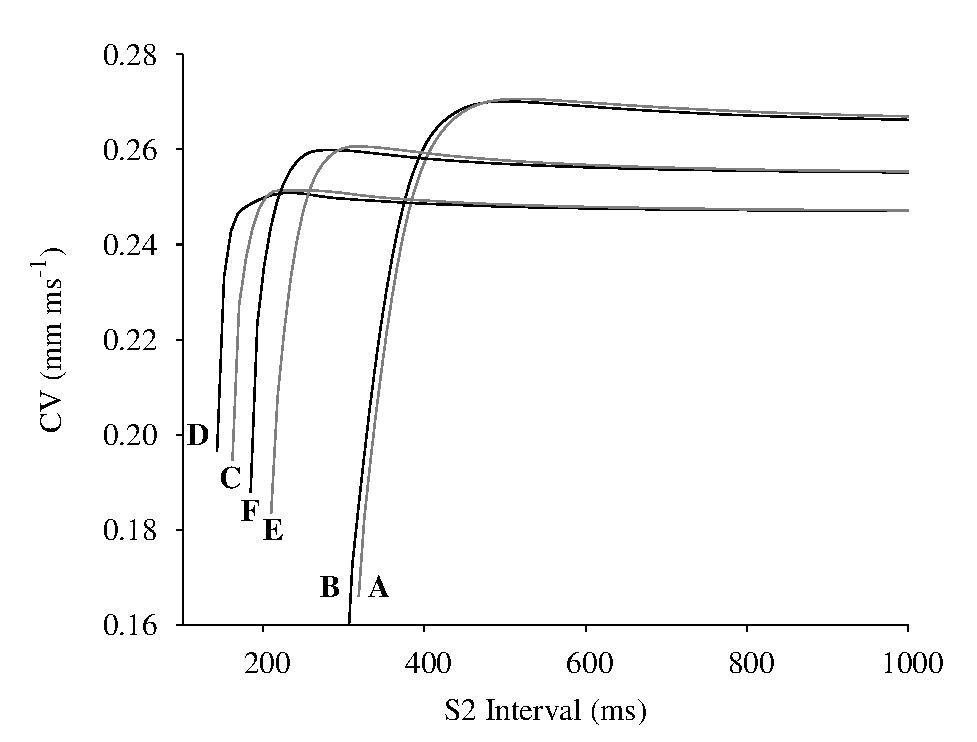
\includegraphics{figures/4_cvr}
\caption{CVr curves for control CT (A), control AM/PM (B), AF1 CT (C),
AF1 AM/PM (D), AF2 CT (E), AF2 AM/PM (F).  In each of the conditions,
the CT cells showed a higher CV at long (1000~ms) S2 intervals, but AM
and PM cells allow faster conduction at shorter S2 intervals.  The AF
cases show reduced CV compared to the control and support a higher
pacing rate via reduced minimum interval.}
\label{fig:cvr}
\end{figure}

Simulations over the 2D geometry examined the lifetime and behavior of
spiral waves in the presence and absence of electrical heterogeneity.
As can be seen in Figure~\ref{fig:plots}, panels Ai and Bi, re-entrant
activity self-terminated in both homogeneous and heterogeneous cases
when due to spiral wave meander over a large tissue region, it
exits the tissue.  Self-termination was much more rapid in the
electrically heterogeneous case, taking \unit{1.31}{s}, compared with
\unit{3.20}{s} in
the homogeneous case.

Conversely, under AF conditions the re-entry persisted after it was
induced for the whole period of the simulation, a lifespan of over \unit{5}{s}.
Under electrically homogeneous conditions, panels Aii and Aiii show a
stable mother rotor rotating anti-clockwise in the tissue.  But in
heterogeneous conditions, as shown in panels Bii and Biii, a similar
mother rotor to the homogeneous cases is visible towards the right of
each frame.  On the left of the frames, the rotor breaks up into
multiple fibrillatory wavelets on the border of the heterogeneous
regions, forming a complex and chaotic pattern of excitation.

\begin{figure*}[t]
\centering
%\includegraphics{figures/figure4}
\caption{Simulation of re-entry in 2D sheets of electrically homogeneous
(A) and electrically heterogeneous (B) sheets.  Columns show
representative frames after initiation of re-entry at t = 0.  Panels i
show data under control conditions, panels ii under AF1 conditions and
panels iii under AF2 conditions.  Re-entry self-terminated under control
conditions in both homogeneous (Ai) and heterogeneous (Bi).  Under AF
conditions, re-entry becomes a sustained mother rotor in
electrically homogeneous conditions (Aii, Aiii).  However, under
electrically heterogeneous conditions AF causes re-entry to degenerate
into erratic propagations on the borders of the heterogeneity (Bii,
Biii).}
\label{fig:plots}
\end{figure*}

\subsubsection{Discussion and conclusions}

AFER induces significant changes in the cellular electrophysiology that
appear to affect rate dependent electrical activities.  It helps to
sustain re-entry, providing evidence to substantiate the hypothesis of
``AF begets AF''.

Considering first the single cell results, one of the most obvious
effects is the striking reduction in the \apd\ and repolarization
properties.  AFER abbreviated \apd\ in AM cells by 66~\% in AF1 and
53~\% in AF2.  Other work has already suggested why the increases shown
in the maximal slope of the APDr can be
pro-arrhythmic~\cite{ByungSoo2002}, as can the reduced
ERP~\cite{Xie2002}.  Our study suggested that reduction is not uniform
across all cell types, which leads to an augmented heterogeneity.

The 1D strand results for the CV tell a similar story.  AFER tissue
forms a much better substrate for arrhythmic activity, supporting both a
much higher maximal pacing rate and in addition, the reduction in
conduction wavelength, to below half the control values. This allows a
greater number of excitation waves to exist in the tissue at any one
time.

The 2D simulations in the realistic sheet show a marked difference in
re-entrant behavior between homogeneous and heterogeneous simulations.
The homogeneous sheets show self-termination of re-entry in control
tissue, whilst the reduced ERP and conduction wavelength allow the rotor
to remain stable and persist for the duration of the simulation in AFER
condtions.  The heterogeneous sheet simulations, show spiral wave
breakup, as observed in real tissue \cite{Kumagai1997}, in both control
and AF simulations, possibly due to elevated plateau potentials and
increased refractory period of the CT cells.  Self-termination is still
observed in control simulations and is more rapid than in homogeneous
tissue.

It is still unclear about the pro- or anti-arrhythmogenic effects of
electrical heterogeneity in the human atria.  Self-termination is more
rapid in the heterogeneous tissue for the control case, but despite AFER
increasing the heterogeneity between tissue types, it doesn't lead to
self termination of the re-entry.  In fact, it leads to breakup of the
spiral wave in the region of the heterogeneity, leading to a region of
erratic propagations, as has been seen in experiment~\cite{Kumagai1997}.
Further study, in both 3D geometries and physiological experiments,
would be needed to elucidate the true effects of the heterogeneity.


